% set the document type and base font size
\documentclass[17pt]{extarticle}

% Geometry package supports custom border and format definitions
\usepackage[a4paper, top=2cm, bottom=2cm, left=2cm, right=2cm]{geometry}
% extsizes package allows to set the base font size to 8-20 pixels (https://ctan.org/pkg/extsizes)
\usepackage{extsizes}
% remove limitation to ascii by introducing UTF8 support 
\usepackage[utf8]{inputenc}
% enables support for the german 'Umlaute': ä, ö, ü
\usepackage[T1]{fontenc}
% mathematical expressions with tabstop support (https://texblog.org/2008/10/01/adding-normal-text-into-formulas/)
\usepackage{amsmath}
% text coloring, obviously
\usepackage{color}
% import and positioning of pictures and graphics
\usepackage{graphicx}
\usepackage{gensymb}
% disable indentation for new paragraphs
\setlength{\parindent}{0pt}

% some neaty shortcuts
%% normalize a vector
\newcommand{\norm}[1]{\lvert #1 \rvert}

% document meta information
\author{Lukas Steiger}
\title{HSR Formelsammlung PhAI}
\date{20.4.17}

% start of the document content
\begin{document}
\begin{center}
	\huge{HSR Formelsammlung PhAI} \\
	\small{Autor: Lukas Steiger}
\end{center}

\tableofcontents
	
\section{Grundlagen - Bewegung und Kräfte}

	Beschleunigung
	\begin{align}
		a = \frac{v^{2}}{2 s}
	\end{align}

	Geschwindigkeit
	\begin{align}
		&v = v_{0} * a * t
		&&v = \sqrt{ v_{0}^2 + 2 a s }
	\end{align}
	
	Lichtgeschwindigkeit
	\begin{align}
		c = 3 * 10^{8} m/s
	\end{align}
	
	Kraft \small{(Newtonsches Bewegungsgesetz)}
	\begin{align}
		&F = m * a
		&&F = m * g
	\end{align}
	
	Schwerkraft \small{(Gravitationskraft)}
	\begin{align}
		&F_{G} = m * g
		&&g = 9.81 \frac{m}{s^{2}} 
	\end{align}
	
	Zurückgelegte Strecke \small{($s_{0}$ oder $v_{0}*t$ weglassen, falls 0)}
	\begin{align}
		&s(t) = s_{0} + v_{0} * t + \frac{a}{2} * t^{2}
		&&\text{\small{oder einfach}}
		&&&s = v * t
	\end{align}
	
	Minimale Strecke, um Abstand nicht zu unterschreiten
	\begin{align}
		s_{0} = D_{min} + \frac{v_{B}^2 t_{A}}{2 v_{A}}
	\end{align}
	
	Endgeschwindigkeit Freier Fall
	\begin{align}
		v = \sqrt{2 g h}
	\end{align}
	
	\section{Bewegung}
	Winkelgeschwindigkeit
	\begin{align}
		\omega = \omega_{0} + at
	\end{align}
	
	Zurückgelegter Radius
	\begin{align}
		\varphi = \omega_{0}t + \frac{a}{2}t^2 = \frac{\omega_{2}^2 - \omega_{1}^2}{2a_{2}}
	\end{align}
	
	\section{Würfe}

	\subsection{Senkrechter Wurf}
	\begin{align}
		y * v_{0} * t - \frac{g}{2} * t^{2}
	\end{align}
	
	Wurfhöhe
	\begin{align}
		h = \frac{v_{0}^{2}}{2g}
	\end{align}
	
	Zeit, bis Geschoss wieder an Ursprungsposition ankommt
	\begin{align}
		t = 2 * \frac{v_{0}}{g} 
	\end{align}
	\subsection{Horizontaler Wurf}
	\begin{align}
		y = - \frac{g}{2v_{0}^{2}} * x^{2}
	\end{align}
	
	Wurfweite
	\begin{align}
		x = \sqrt{\frac{2 * v_0^2 * y}{g}}
	\end{align}
	
	\subsection{Schiefer Wurf}
	\begin{align}
		y(x) = x * \tan \varphi - \frac{g}{2 * v_{0}^{2} * \cos^{2} \varphi} * x^{2}
	\end{align}
	
	Wurfhöhe
	\begin{align}
		y_{max} = \frac{v_{0}^{2} * \sin^{2} \varphi}{2g}
	\end{align}
	
	Wurfweite
	\begin{align}
		&d = \frac{v_{0}^{2} * \sin(2\varphi)}{g}
		&&d_{max}: \alpha = 45\degree
	\end{align}


\section{Vektoren}
	Normalenvektor
	\begin{align}
		&\vec{n} =
		\begin{pmatrix} a \\ b \\ c \end{pmatrix}		
		&&wenn: ax + by + cz + d = 0
	\end{align}
	
	Normalenvektor skalieren
	\begin{align}
		\vec{n} = \frac{1}{\norm{\vec{w}}} \vec{w}
	\end{align}

	Addition / Subtraktion
	\begin{align}	
		\vec{a} \pm \vec{b} = 
		\begin{pmatrix} a_x \\ a_y \end{pmatrix}
		\pm
		\begin{pmatrix} b_x \\ b_y \end{pmatrix}
		=
		\begin{pmatrix} a_x \pm b_x \\ a_y \pm b_y \end{pmatrix}
	\end{align}
	
	Skalarprodukt 	
	\begin{align}	
	\vec{a} * \vec{b} = 
	\begin{pmatrix} a_x \\ a_y \end{pmatrix}
	*
	\begin{pmatrix} b_x \\ b_y \end{pmatrix}
	= a_x * b_x + a_y * b_y
	\end{align}
	
	Betrag / Länge / Fläche
	\begin{align}
		\norm{\vec{a}} = \sqrt{a_x^2 + a_y^2}
	\end{align}
	
	Winkel zwischen zwei Vektoren
	\begin{align}
		&\cos \phi = \frac{\vec{a} * \vec{b}}{\norm{\vec{a}} \norm{\vec{b}}}
		&&\phi = \arctan(\cos \phi)
	\end{align}
	
	Vektorprodukt / Kreuzprodukt
	\begin{align}
		\vec{a} x \vec{b} = 
		\begin{pmatrix} a_x \\ a_y \\ a_z \end{pmatrix}
		x
		\begin{pmatrix} b_x \\ b_y \\ b_z \end{pmatrix}
		=
		\begin{pmatrix} a_y b_z - a_z b_y \\ a_z b_x - a_x b_z \\ a_x b_y - a_y b_x \end{pmatrix}
	\end{align}
	
\section{Kräfte, Arbeit, Leistung \& Energie}
	\begin{figure}[h!]
		\centering
		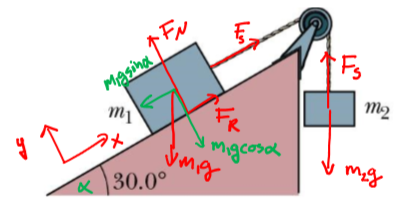
\includegraphics[width=12cm]{img/Haftreibung.png}
	\end{figure}

	Steigungswinkel
	\begin{align}
		\alpha = \arctan(\frac{S}{100\%}) 
	\end{align}
		
	Maximale Haftreibung
	\begin{align}
		&F_{R,max} = \mu_{H} * F_{N}
		&&\mu_{H} = \text{Haftreibungskoeffizient} 
	\end{align}

	Konstante Gleitreibung
	\begin{align}
		&F = \mu_{G} * F_{N}
		&&\mu_{G} = \text{Gleitreibungskoeffizient}		
	\end{align}

	Mechanische Arbeit \small{($1J = 1Nm = \frac{1*kg m^{2}}{s^{2}} | 1 kWh = 3.6 * 10^6$)}
	\begin{align}
		W = F * s
	\end{align}
	\begin{align}
		W = m g h = \varrho V g h = (\sin \alpha + \mu_R \cos \alpha) * F_G s = (1 + \mu * (1/\tan \alpha)) * F_G * h
	\end{align}

	Energieerhaltung
	\begin{align}
		E_{pot} + E_{kin} = \text{konstant}
	\end{align}
	
	Potentielle Energie
	\begin{align}
		&\text{geleistete Arbeit} 
		&&W = E_{pot} 
		&&&\text{potentielle Energie}
	\end{align}
	
	Kinetische Energie
	\begin{align}
		E_{kin} = \frac{1}{2} * m * v^{2}
	\end{align}
	
	Federkraft
	\begin{align}
		F = k * s
	\end{align}
	
	Federenergie
	\begin{align}
		&E_{pot} = \frac{1}{2} * k * x^{2}
		&&k = Federkonstante [N/m]
		&&&x = Ausdehnung Feder
	\end{align}
	
	Wärmeenergie
	\begin{align}
		&Q = \frac{\mu * v_R^2}{2}
		&&\mu = \frac{m_1 m_2}{m_1 + m_2}
		&&&v_R = v_1 - v_2
	\end{align}
	
	Leistung \small(Arbeit pro Zeiteinheit in $J/s = W | 1kW = 1.36 PS$ )
	\begin{align}
		P = \frac{\Delta W}{\Delta t} = F * v = m * a^{2} * t
	\end{align}
	
	Impuls / Gesamtimpuls
	\begin{align}
		&p = m * v = F * \Delta t
		&&P = p_{1} + p_{2} + ... + p_{n}
	\end{align}
	
	Schwerpunktgeschwindigkeit
	\begin{align}
		u = \frac{p_{1} + p_{2} + ... + p_{n}}{m_{1} + m_{2} + ... + m_{n}}
	\end{align}
	
	Zentripetalkraft (nach innen gerichtet)
	\begin{align}
		&F_Z = \frac{m v^2}{r}
		&& r = Radius (Länge)
	\end{align}
	
	Umlaufzeit [s]
	\begin{align}
		T = \frac{2 \pi}{\omega}  = \frac{1}{f}
	\end{align}
	
	Frequenz [1/s]
	\begin{align}
		f = \frac{1}{T} = \frac{\omega}{2 \pi}
	\end{align}
	
	Zentrifugalkraft (nach aussen gerichtet)
	\begin{align}
		&F = m * \frac{v^2}{r} = m r \omega^2 = \frac{m * 4 \pi^2 * r}{T^2}
		&&\omega = 2 \pi f
	\end{align}
	\begin{align}
		& f = Frequenz [1/s]
		&& r = Radius (Länge)
	\end{align}
	
	Gravitationskonstante
	\begin{align}
		G = 6.672 * 10^{11} \frac{m^3}{kg*s^2}
	\end{align}
	
	Gravitationskraft
	\begin{align}
		&F = \frac{G * m * M}{r^2}
		&&m: 1. Masse, M: 2. Masse
		&&&r: Abstand zwischen Massepunkten
	\end{align}
	
\section{Dynamik}
	Drehmoment
	\begin{figure}[h!]
		\centering
		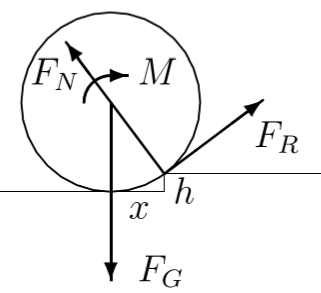
\includegraphics[width=4cm]{img/Drehmoment.png}
	\end{figure}

	\begin{align}
		&M = x*F_{G}
		&&x = \sqrt{2rh - h^2}
	\end{align}
	
	\begin{align}
		&M = J \alpha
		&&J = Traegheitsmoment
		&&&\alpha = Winkelbeschleunigung
	\end{align}
	
	Rotationsgeschwindigkeit
	\begin{align}
		\omega = \omega_{0} + \alpha * t = \omega_{0} + \frac{M}{J} * t
	\end{align}
	
	Drehzahl [$\frac{1}{s}$]
	\begin{align}
		\upsilon = \frac{\omega}{2 * \pi} = \upsilon_{0} + \frac{M}{2\pi * J} * t 
	\end{align}
	
	Anzahl Umdrehungen
	\begin{align}
		U = \frac{\upsilon * 2 \pi * t + \frac{a}{2} * t^2}{2 \pi}
	\end{align}
	
	Drehimpuls 
	\begin{align}
		L = J * \omega
	\end{align}
	
	Rotationsenergie
	\begin{align}
		E_{rot} = \frac{J}{2} \omega^2
	\end{align}
	
	Leistung bei Rotation
	\begin{align}
		P = M * \omega
	\end{align}
	
	Druck (= Kraft pro Fläche)
	\begin{align}
		p = \frac{F}{A}
	\end{align}	
	
	Schweredruck 
	\begin{align}
		&\Delta p = p_0 * \varrho g \Delta h
		&&p_0 z.B. Luftdruck 
		&&&1 bar = 100'000 Pa
	\end{align}
	
	Gesamtdruck
	\begin{align}
		p_{ges} = \frac{p}{2}v^2 + pgh + p_{st}
	\end{align}
	\begin{align}		
		Gesamtdruck = Staudruck + Schweredruck + statischer Druck
	\end{align}

	Horizontale Krafteinwirkung auf eine Fläche
	\begin{align}
		F = A * \overline{\Delta p} = b*h * \varrho*g (h_{0} + \frac{h}{2})
	\end{align}
	
	
\section{Thermodynamik}
	


	Laminare Strömung im Rohr (Hagen Poiseuille)
	\begin{align}
		V = \frac{\pi * \Delta p * t * R^4}{8 * \eta * l}
	\end{align}
	\begin{align}
		&V: \text{Volumen der Flüssigkeit}
		&&R: \text{Radius des Rohres}
		&&&\Delta p: \text{Druckdifferenz Rohrenden}
	\end{align}
	\begin{align}
		&&&&t: \text{Dauer des Flusses}
		&&&&&l: \text{Rohrlänge}
		&&&&&&\eta: \text{dyn. Viskosität (konst.)}
	\end{align}
	
	Reynoldszahl
	\begin{align}
		&Re_k = \frac{d* \varrho * v}{\eta}
		&&d: \text{char. Länge (z.B. Rohrradius)}
	\end{align}

	Termperatureinheiten
	\begin{align}
		&T_{Kelvin} = T_{Celsius} + 273.15
		&&T_{Fahrenheit} = T_{Celsius} * 1.8 + 32
	\end{align}


\subsection{Molare Grössen}
	\begin{align}
		&n: \text{Stoffmenge}
		&&v: \text{spez. Volumen = V/m}
		&&&p: \text{Absolutdruck}
	\end{align}
	\begin{align}
		&N: \text{Anzahl Teilchen}
		&&T: \text{Temperatur in Kelvin}
	\end{align}
	\begin{align}
		k_B: \text{Boltzmann K. =} 1.381 * 10^{-23}
	\end{align}
	\begin{align}		
		R: \text{Gas K. =} k_B * N_A = 8.314 J/mol K
	\end{align}
	\begin{align}
		N_A: \text{Avogadro K. =} 6.02 * 10^{23} mol-1
	\end{align}

	molare Masse [kg/mol]
	\begin{align}
		M = \frac{m}{n}
	\end{align}

	molares Volumen [$m^3/mol$]
	\begin{align}
		V_m = \frac{V}{n}
	\end{align}
	
	stoffbezogene Zustandsgleichung
	\begin{align}
		pV = n R T = N k_B T
	\end{align}
	
\section{Repetition - Trigonometrie}
	\begin{align}
		\sin \alpha = \frac{a}{c} = \pm \sqrt{1 - \cos^2 \alpha}
	\end{align}
	\begin{align}
		\cos \alpha = \frac{b}{c} = \pm \sqrt{1 - \sin^2 \alpha}
	\end{align}
	\begin{align}
		\tan \alpha = \frac{a}{b} = \frac{\sin \alpha}{\cos \alpha}
	\end{align}
	\begin{figure}[h!]
		\centering
		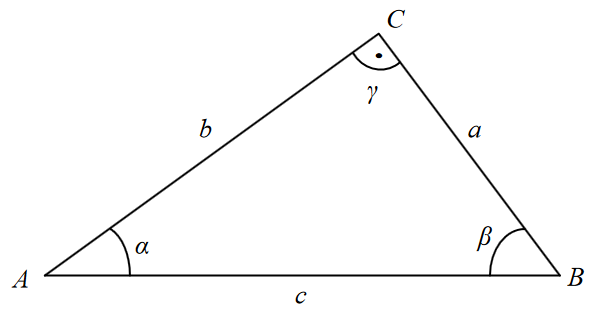
\includegraphics[width=10cm]{img/Trigonometrie.png}
	\end{figure}
	
	Trigonometrischer Pythagoras
	\begin{align}
		\cos^2 \alpha + \sin^2 \alpha = 1
	\end{align}

	Additionstheoreme
	\begin{align}
		\sin(\alpha \pm \beta) = \sin(\alpha) \cos(\beta) \pm \cos(\alpha) \sin(\beta)
	\end{align}
	\begin{align}
		\sin(\alpha \pm \beta) = \cos(\alpha) \cos(\beta) \mp \sin(\alpha) \sin(\beta)
	\end{align}

\section{Anhang}
	\subsection{Periodensystem}
	\begin{figure}[h!]
		\centering
		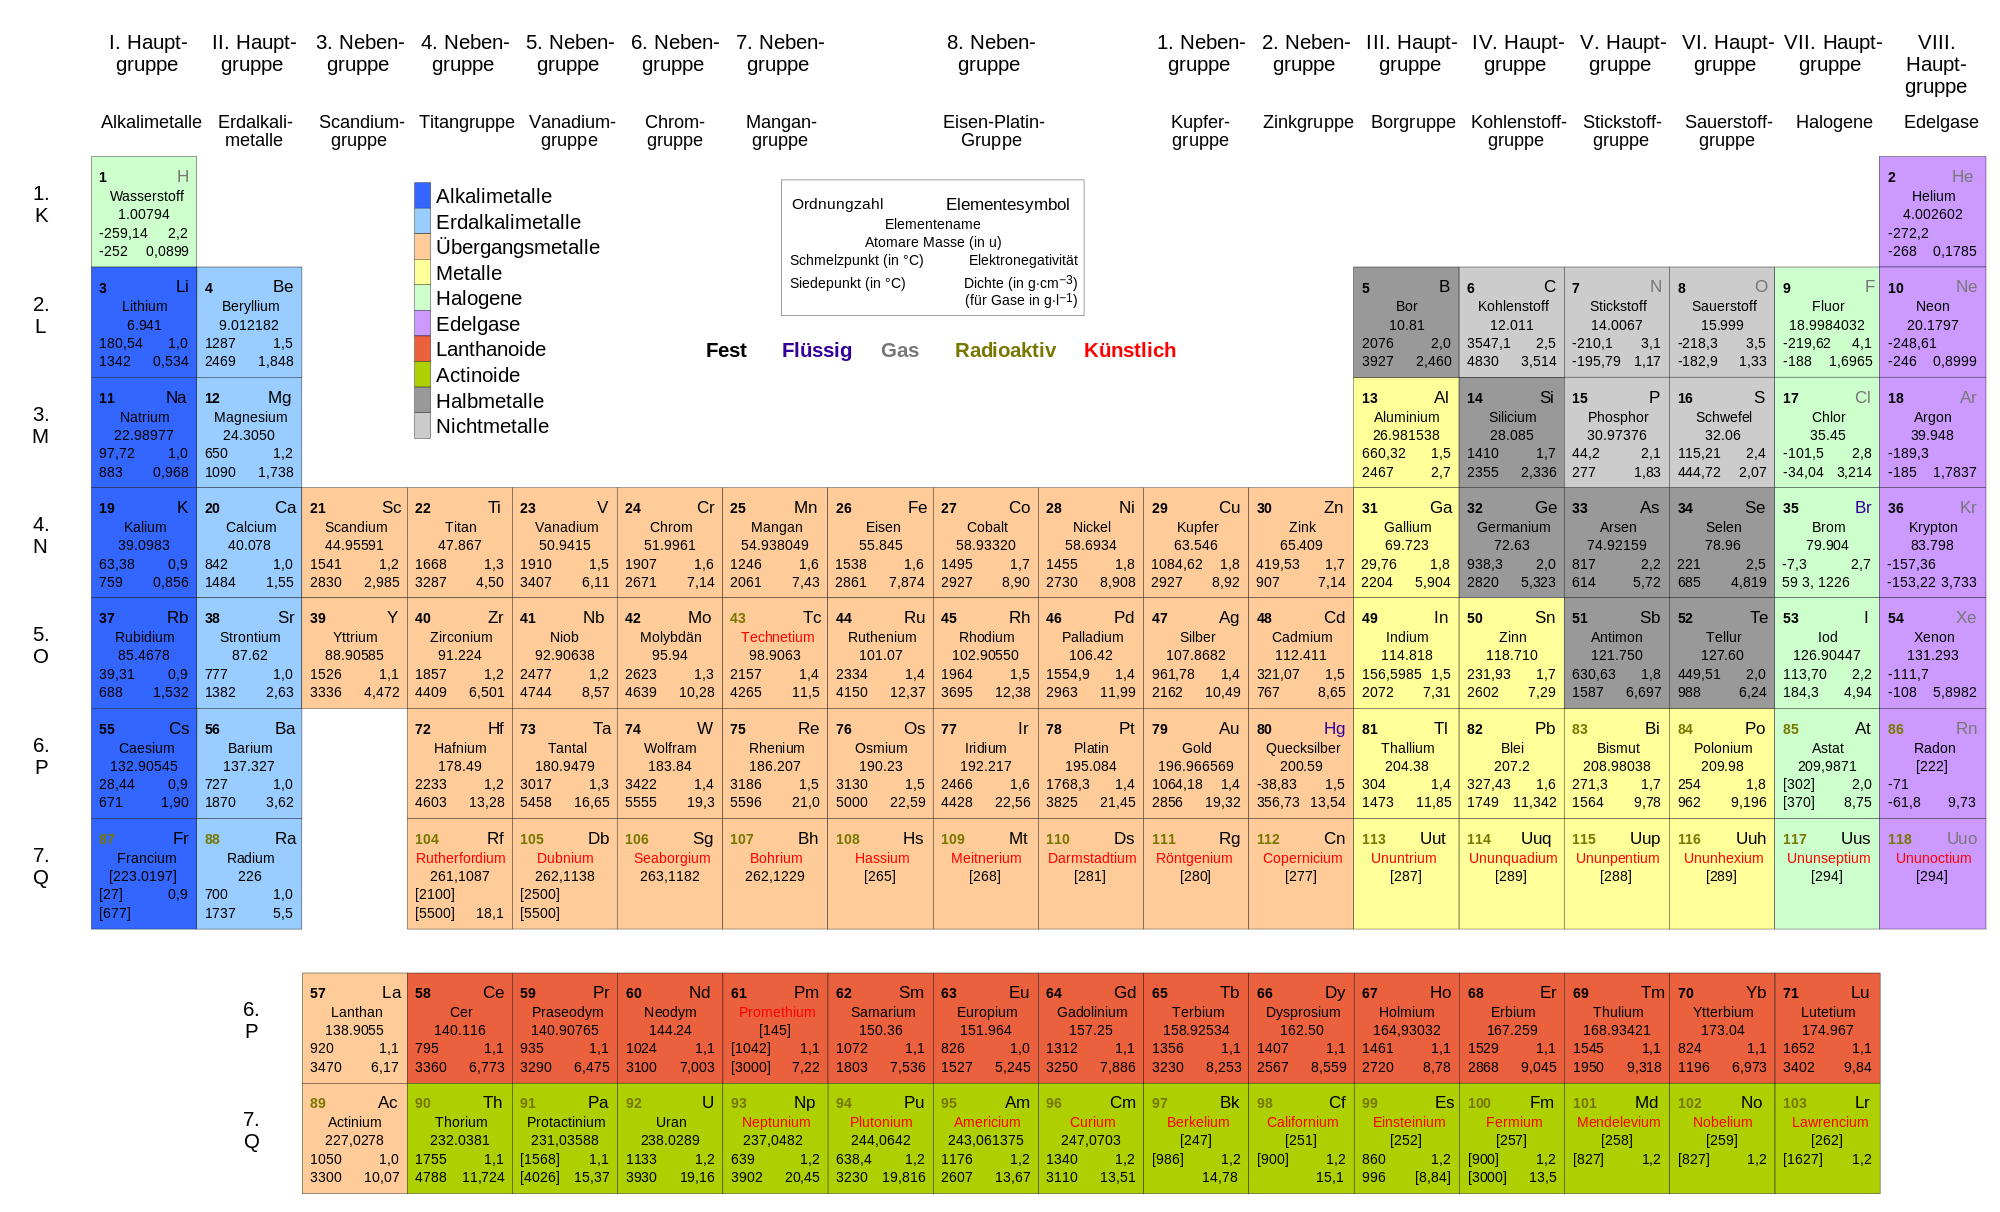
\includegraphics[width=25cm, angle=90]{img/Periodensystem.png}
	\end{figure}

\end{document}